\documentclass[conference]{IEEEtran}

\usepackage[utf8]{inputenc}
\usepackage[T1]{fontenc}
\usepackage{amsmath,amssymb}
\usepackage{graphicx}
\usepackage{tikz}
\usetikzlibrary{positioning, arrows.meta, shapes.geometric, fit, calc, decorations.pathreplacing}
\usepackage{listings}
\usepackage{xcolor}
\usepackage{hyperref}
\usepackage{booktabs}
\usepackage{pifont}
\usepackage{algorithm}
\usepackage{algorithmic}
\usepackage{balance}

\lstset{
  language=Python,
  basicstyle=\ttfamily\scriptsize,
  keywordstyle=\color{blue}\bfseries,
  commentstyle=\color{gray},
  stringstyle=\color{red!60!black},
  showstringspaces=false,
  frame=single,
  breaklines=true,
  captionpos=b,
}

\hypersetup{colorlinks=true, linkcolor=blue, citecolor=blue, urlcolor=blue}

\title{lix\_cache: A Multi-Layer Caching Architecture\\for Conversational AI Session Management}

\author{
\IEEEauthorblockN{Elixpo Research}
\IEEEauthorblockA{search.elixpo.com}
}

\begin{document}

\maketitle

% ============================================================
% ABSTRACT
% ============================================================
\begin{abstract}
Conversational AI systems face a persistent tension between response latency and contextual fidelity. As dialogue sessions grow, maintaining a responsive user experience while preserving conversation history becomes increasingly expensive. We present \texttt{lix\_cache}, an open-source, pip-installable Python library that addresses this problem through a three-layer caching architecture built on Redis and compressed disk storage. The system comprises: (1)~a \emph{Session Context Window} that maintains a rolling window of recent messages in Redis with automatic overflow to Huffman-compressed disk archives; (2)~a \emph{Semantic Query Cache} that eliminates redundant LLM invocations by matching incoming queries against cached responses using cosine similarity on embedding vectors; and (3)~a \emph{URL Embedding Cache} that deduplicates embedding computations across sessions. A background LRU eviction daemon transparently migrates idle sessions from Redis to disk and re-hydrates them on demand. We describe the architecture, design rationale, and implementation of each layer, present a custom binary \texttt{.huff} file format for conversation archival, and evaluate the system's compression efficiency, cache hit rates, and latency characteristics. The library is extracted from the production lixSearch system and is designed for drop-in integration with any chatbot, search assistant, or RAG pipeline.
\end{abstract}

\begin{IEEEkeywords}
caching, conversational AI, session management, Redis, Huffman coding, semantic similarity, embedding cache, RAG
\end{IEEEkeywords}

% ============================================================
% I. INTRODUCTION
% ============================================================
\section{Introduction}

Modern conversational AI applications---chatbots, search assistants, and retrieval-augmented generation (RAG) pipelines---must solve three recurring problems simultaneously:

\begin{enumerate}
\item \textbf{``What did we just talk about?''} Users expect the system to recall recent conversation context. Na\"ive approaches store entire histories in memory, which does not scale across thousands of concurrent sessions.

\item \textbf{``Didn't we already answer this?''} Semantically equivalent queries arrive frequently, especially in multi-turn dialogues where users rephrase or refine earlier questions. Each redundant LLM invocation wastes compute and adds latency.

\item \textbf{``We already embedded this URL.''} In RAG workflows, the same URLs are fetched and embedded by multiple sessions. Re-computing a 384-dimensional embedding vector (${\sim}200$\,ms per URL) for every session is wasteful when the content has not changed.
\end{enumerate}

Existing solutions typically address one of these concerns in isolation: frameworks like LangChain~\cite{langchain2023} provide memory modules for conversation history, while GPTCache~\cite{gptcache2023} focuses on semantic caching of LLM responses. However, no single, lightweight library unifies session management, semantic query deduplication, and embedding caching into a cohesive, production-ready package with minimal dependencies.

We present \texttt{lix\_cache}, a Python library extracted from the production \texttt{lixSearch} intelligent search assistant. The library provides:

\begin{itemize}
\item A \textbf{three-layer caching architecture} where each layer targets a distinct problem (session context, query deduplication, embedding reuse) and operates on a separate Redis logical database.
\item A \textbf{two-tier hybrid storage model} combining Redis for hot data (${\sim}1$\,ms reads) with Huffman-compressed disk archives for cold data, connected by a background LRU eviction daemon.
\item A \textbf{custom binary file format} (\texttt{.huff}) with a fixed 24-byte header and canonical Huffman-coded payload, achieving ${\sim}54\%$ compression on typical conversation text with zero native dependencies.
\item A \textbf{single \texttt{CacheConfig} dataclass} that centralizes all tunables and supports 12-factor environment variable loading.
\end{itemize}

The library is pip-installable (\texttt{pip install lix-chat}), requires only \texttt{redis}, \texttt{numpy}, and \texttt{loguru} as dependencies, and is designed for drop-in integration with any Python-based conversational system.

The remainder of this paper is organized as follows. Section~\ref{sec:architecture} presents the overall system architecture and data flow. Section~\ref{sec:design} discusses key design decisions and their rationale. Section~\ref{sec:implementation} details the implementation of each component. Section~\ref{sec:evaluation} evaluates compression ratios, latency, and cache hit behavior. Section~\ref{sec:related} surveys related work, and Section~\ref{sec:conclusion} concludes.

% ============================================================
% II. ARCHITECTURE
% ============================================================
\section{Architecture}
\label{sec:architecture}

\subsection{Overview}

The \texttt{lix\_cache} system is organized as three independent caching layers, each backed by a dedicated Redis logical database, unified under a single \texttt{CacheCoordinator} fa\c{c}ade. Figure~\ref{fig:architecture} illustrates the complete data flow when a user message arrives.

\begin{figure*}[t]
\centering
% TikZ Architecture Diagram — redesigned to fit single column width (~3.5in)
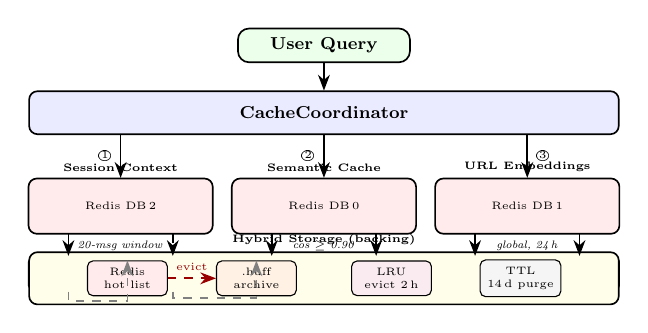
\begin{tikzpicture}[
    scale=0.78, transform shape,
    node distance=0.5cm and 0.6cm,
    >=Stealth,
    every node/.style={font=\footnotesize},
    layer/.style={draw, rounded corners=3pt, minimum width=3.0cm, minimum height=0.9cm, align=center, semithick},
    sublayer/.style={draw, rounded corners=2pt, minimum width=1.3cm, minimum height=0.55cm, align=center, font=\tiny, thin},
    redis/.style={fill=red!8},
    disk/.style={fill=orange!10},
    coord/.style={fill=blue!8},
    arrow/.style={->, semithick, >=Stealth},
    dasharrow/.style={->, semithick, dashed, >=Stealth},
]

% ── User message ──
\node[draw, rounded corners=4pt, fill=green!8, minimum width=2.8cm, minimum height=0.55cm, semithick]
    (user) {\textbf{User Query}};

% ── CacheCoordinator ──
\node[draw, rounded corners=3pt, coord, below=0.45cm of user, minimum width=9.6cm, minimum height=0.7cm, semithick]
    (coordinator) {\textbf{CacheCoordinator}};

% ── Three layers side by side ──
\node[layer, redis, below=0.7cm of coordinator.south west, anchor=north, xshift=1.5cm]
    (session) {};
\node[above=-0.02cm, font=\tiny\bfseries] at (session.north) {Session Context};
\node[font=\tiny] at (session.center) {Redis DB\,2};
\node[below=-0.02cm, font=\tiny] at (session.south) {\textit{20-msg window}};

\node[layer, redis, below=0.7cm of coordinator.south, anchor=north]
    (semantic) {};
\node[above=-0.02cm, font=\tiny\bfseries] at (semantic.north) {Semantic Cache};
\node[font=\tiny] at (semantic.center) {Redis DB\,0};
\node[below=-0.02cm, font=\tiny] at (semantic.south) {\textit{cos $\geq$ 0.90}};

\node[layer, redis, below=0.7cm of coordinator.south east, anchor=north, xshift=-1.5cm]
    (urlcache) {};
\node[above=-0.02cm, font=\tiny\bfseries] at (urlcache.north) {URL Embeddings};
\node[font=\tiny] at (urlcache.center) {Redis DB\,1};
\node[below=-0.02cm, font=\tiny] at (urlcache.south) {\textit{global, 24\,h}};

% ── Sub-nodes: Session hot/cold ──
\node[sublayer, redis, below=0.35cm of session.south, xshift=-0.85cm]
    (hot) {\textbf{Hot}\\Redis};
\node[sublayer, disk, below=0.35cm of session.south, xshift=0.85cm]
    (cold) {\textbf{Cold}\\.huff};

% ── Sub-nodes: Semantic hit/miss ──
\node[sublayer, fill=green!10, below=0.35cm of semantic.south, xshift=-0.85cm]
    (semhit) {HIT\\skip LLM};
\node[sublayer, fill=yellow!10, below=0.35cm of semantic.south, xshift=0.85cm]
    (semmiss) {MISS\\call LLM};

% ── Sub-nodes: URL hit/miss ──
\node[sublayer, fill=green!10, below=0.35cm of urlcache.south, xshift=-0.85cm]
    (urlhit) {HIT\\$\sim$0\,ms};
\node[sublayer, fill=yellow!10, below=0.35cm of urlcache.south, xshift=0.85cm]
    (urlmiss) {MISS\\embed};

% ── Hybrid backing store ──
\node[draw, rounded corners=3pt, fill=yellow!8, minimum width=9.6cm, minimum height=0.85cm, semithick,
      below=1.9cm of coordinator.south, anchor=north]
    (hybrid) {};
\node[above=-0.02cm, font=\tiny\bfseries] at (hybrid.north) {Hybrid Storage (backing)};

\node[sublayer, redis, at=(hybrid.center), xshift=-3.2cm]
    (hybhot) {Redis\\hot list};
\node[sublayer, disk, at=(hybrid.center), xshift=-1.1cm]
    (hybcold) {.huff\\archive};
\node[sublayer, fill=purple!8, at=(hybrid.center), xshift=1.1cm]
    (hyblru) {LRU\\evict 2\,h};
\node[sublayer, fill=gray!8, at=(hybrid.center), xshift=3.2cm]
    (hybttl) {TTL\\14\,d purge};

% ── Arrows ──
\draw[arrow] (user.south) -- (coordinator.north);

\draw[arrow] (coordinator.south -| session.north) -- (session.north)
    node[midway, left, font=\tiny] {\textcircled{\tiny 1}};
\draw[arrow] (coordinator.south) -- (semantic.north)
    node[midway, left, font=\tiny] {\textcircled{\tiny 2}};
\draw[arrow] (coordinator.south -| urlcache.north) -- (urlcache.north)
    node[midway, right, font=\tiny] {\textcircled{\tiny 3}};

\draw[arrow] (session.south -| hot.north) -- (hot.north);
\draw[dasharrow] (session.south -| cold.north) -- (cold.north);

\draw[arrow] (semantic.south -| semhit.north) -- (semhit.north);
\draw[arrow] (semantic.south -| semmiss.north) -- (semmiss.north);

\draw[arrow] (urlcache.south -| urlhit.north) -- (urlhit.north);
\draw[arrow] (urlcache.south -| urlmiss.north) -- (urlmiss.north);

\draw[dasharrow, gray] (hot.south) -- ++(0,-0.15) -| (hybhot.north);
\draw[dasharrow, gray] (cold.south) -- ++(0,-0.1) -| (hybcold.north);

\draw[dasharrow, red!60!black] (hybhot.east) -- (hybcold.west)
    node[midway, above, font=\tiny, red!60!black] {evict};

\end{tikzpicture}

\caption{Data flow through the three-layer caching architecture. Solid arrows indicate the primary path; dashed arrows indicate overflow and eviction paths.}
\label{fig:architecture}
\end{figure*}

\subsection{Layer 1: Session Context Window (Redis DB\,2)}

The Session Context Window maintains a rolling window of the $k$ most recent messages (default $k{=}20$) for each session. Messages are stored as individual Redis keys with TTL, and an ordered list tracks message insertion order.

When a new message arrives, it is pushed to the head of the Redis list. If the list exceeds $k$ entries, the oldest message is popped, serialized, and appended to a Huffman-compressed disk archive. This ensures Redis memory usage remains bounded at $O(k)$ per session regardless of conversation length.

When \texttt{get\_context()} is called and Redis is empty (e.g., after LRU eviction), the system transparently re-hydrates by loading the last $k$ messages from the disk archive back into Redis. If Redis is entirely unavailable, the system falls back to disk-only reads.

\subsection{Layer 2: Semantic Query Cache (Redis DB\,0)}

The Semantic Query Cache intercepts queries before they reach the LLM. For each incoming query, the system:

\begin{enumerate}
\item Computes an embedding vector $\mathbf{q} \in \mathbb{R}^{384}$ for the query.
\item Retrieves all cached $(\mathbf{e}_i, r_i)$ pairs for the current session and URL, where $\mathbf{e}_i$ is a cached embedding and $r_i$ the corresponding LLM response.
\item Computes cosine similarity: $\text{sim}(\mathbf{q}, \mathbf{e}_i) = \frac{\mathbf{q} \cdot \mathbf{e}_i}{\|\mathbf{q}\| \|\mathbf{e}_i\|}$.
\item If $\max_i \text{sim}(\mathbf{q}, \mathbf{e}_i) \geq \tau$ (default $\tau{=}0.90$), returns the cached response $r_i$ and skips the LLM entirely.
\end{enumerate}

This catches rephrasings: ``weather Tokyo'' versus ``Tokyo weather forecast'' typically yields $\text{sim} \approx 0.94$, producing a cache hit. Each URL stores up to 50 cached pairs (configurable), with a 5-minute TTL to balance freshness against hit rate. Cache entries are scoped per-session for privacy isolation.

\subsection{Layer 3: URL Embedding Cache (Redis DB\,1)}

The URL Embedding Cache is a global (cross-session) store mapping URL strings to their pre-computed embedding vectors, stored as raw \texttt{float32} byte arrays. Computing an embedding costs ${\sim}200$\,ms per URL via the sentence-transformers model; this cache ensures each URL is embedded at most once per 24-hour window across all sessions.

\subsection{CacheCoordinator}

The \texttt{CacheCoordinator} class serves as the unified entry point. It instantiates all three layers from a shared \texttt{CacheConfig} and exposes a flat API surface:

\begin{itemize}
\item \texttt{add\_message\_to\_context(role, content)} --- delegates to Layer~1
\item \texttt{get\_semantic\_response(url, embedding)} --- delegates to Layer~2
\item \texttt{get\_url\_embedding(url)} --- delegates to Layer~3
\item \texttt{get\_stats()} --- aggregates statistics from all layers
\end{itemize}

This design allows consumers to interact with a single object per session, while each layer remains independently testable and replaceable.

\subsection{Redis Database Separation}

Each layer operates on a separate Redis logical database (DB\,0, DB\,1, DB\,2) rather than using key prefixes within a single database. This provides three operational advantages:

\begin{enumerate}
\item \textbf{Selective flushing}: \texttt{FLUSHDB} on one layer does not affect others.
\item \textbf{Independent monitoring}: \texttt{DBSIZE} and \texttt{INFO} statistics are per-database.
\item \textbf{Namespace isolation}: Eliminates the risk of key collisions between layers.
\end{enumerate}

% ============================================================
% III. DESIGN DECISIONS
% ============================================================
\section{Design Decisions}
\label{sec:design}

\subsection{Three Separate Layers vs.\ a Monolithic Cache}

An alternative design would combine all caching into a single Redis namespace with compound keys. We opted for three independent layers for several reasons:

\begin{itemize}
\item \textbf{Different TTL profiles.} Session context needs long TTLs (24\,h) since users may return to a conversation hours later. Semantic query caches need short TTLs (5\,min) to ensure freshness of LLM-generated content. URL embeddings sit between (24\,h) because web content changes slowly. A monolithic cache would require per-key TTL management at the application level rather than leveraging Redis database-level semantics.

\item \textbf{Different scope.} Session context and semantic caches are per-session (privacy isolation). The URL embedding cache is deliberately global---sharing embedding work across sessions is a key performance optimization.

\item \textbf{Independent failure modes.} If the semantic cache Redis DB is flushed (e.g., during maintenance), conversation history in DB\,2 is unaffected. This partial-failure tolerance simplifies operations.
\end{itemize}

\subsection{Huffman Coding vs.\ gzip/zlib/lz4}

For the disk archive, we chose a custom canonical Huffman codec over standard compression libraries. This decision was driven by three factors:

\begin{enumerate}
\item \textbf{Small payload efficiency.} Conversation archives are typically 1--100\,KB. At these sizes, gzip's dictionary overhead (32\,KB window) and lz4's frame header can dominate. Huffman coding has no dictionary---only a symbol table proportional to the alphabet size (at most 256 entries, $\leq$512 bytes of overhead).

\item \textbf{Exploiting byte frequency skew.} English-language conversation text exhibits extreme byte frequency imbalance: spaces account for ${\sim}18\%$ of bytes, \texttt{`e'} for ${\sim}13\%$, while \texttt{`z'} appears only ${\sim}0.07\%$ of the time. Huffman coding directly exploits this skew, assigning shorter bit codes to frequent bytes.

\item \textbf{Zero native dependencies.} The codec is pure Python (${\sim}160$ lines), eliminating build-time dependencies on C libraries. This is critical for a pip-installable package targeting diverse deployment environments.
\end{enumerate}

The resulting compression achieves ${\sim}54\%$ ratio on typical conversation text (i.e., compressed size is 54\% of original), comparable to zlib level-1 but without native code.

\subsection{Rolling Window with Overflow vs.\ Truncation}

Many conversation memory systems simply truncate: they keep the last $k$ messages and discard everything older. \texttt{lix\_cache} instead \emph{overflows} old messages to disk. This preserves the full conversation history for:

\begin{itemize}
\item \textbf{Semantic retrieval:} The \texttt{smart\_context()} method retrieves semantically relevant messages from the disk archive via embedding cosine similarity, even if those messages left the hot window long ago.
\item \textbf{Audit and replay:} Full history can be reconstructed via \texttt{get\_full\_history()} by merging hot and cold stores.
\item \textbf{Session resumption:} If a user returns after hours (post-eviction), the full archive is available for re-hydration.
\end{itemize}

\subsection{LRU Eviction as a Background Daemon}

Idle session data in Redis consumes memory without serving reads. Rather than relying solely on Redis TTL expiry (which discards data), the LRU daemon \emph{migrates} data to disk before freeing Redis memory. This preserves data while reclaiming resources.

The daemon runs as a Python \texttt{threading.Thread} (daemon mode), checking every 60 seconds for sessions idle longer than the configured threshold (default 120 minutes). It is started lazily on first \texttt{HybridConversationCache} instantiation and shared across all sessions via module-level state.

\subsection{Connection Pooling Strategy}

Redis connections are pooled globally, keyed by the tuple \texttt{(host, port, db)}. The pool is created on first access and reused for all subsequent \texttt{create\_redis\_client()} calls with matching parameters. This ensures that even when hundreds of \texttt{CacheCoordinator} instances are created (one per session), the number of Redis connections remains bounded by \texttt{redis\_pool\_size} (default 50) per database.

Authentication is handled gracefully: the pool first attempts to connect with the configured password, and on \texttt{AuthenticationError} falls back to no-auth. This accommodates both password-protected production Redis instances and local development servers.

\subsection{Single Configuration Object}

All tunables are consolidated into a single \texttt{CacheConfig} dataclass with sensible defaults. This avoids the anti-pattern of scattered magic numbers across service files. The \texttt{from\_env(prefix)} class method supports 12-factor apps by reading environment variables like \texttt{MYAPP\_REDIS\_HOST}, \texttt{MYAPP\_SEMANTIC\_TTL\_SECONDS}, etc.

% ============================================================
% IV. IMPLEMENTATION
% ============================================================
\section{Implementation}
\label{sec:implementation}

The library is implemented in ${\sim}800$ lines of Python across eight modules. We describe the key implementation details of each component.

\subsection{Package Structure}

\begin{lstlisting}[caption={Module layout},label=lst:layout]
lix_chat/
  lix_cache/
    config.py            # CacheConfig dataclass
    redis_pool.py        # Connection-pooled Redis factory
    huffman_codec.py     # Canonical Huffman encoder/decoder
    conversation_archive.py  # .huff disk persistence
    hybrid_cache.py      # Redis hot + disk cold + LRU
    semantic_cache.py    # SemanticCacheRedis + URLEmbeddingCache
    context_window.py    # SessionContextWindow wrapper
    coordinator.py       # CacheCoordinator facade
\end{lstlisting}

All public classes are re-exported through \texttt{lix\_chat/\_\_init\_\_.py}, giving users a flat import surface (e.g., \texttt{from lix\_chat import CacheCoordinator}).

\subsection{Huffman Codec}

The codec implements canonical Huffman coding in pure Python. The encoding process follows three steps:

\begin{enumerate}
\item \textbf{Frequency counting and tree construction.} Byte frequencies are tallied in a single pass. A min-heap builds the Huffman tree, producing code lengths for each symbol.

\item \textbf{Canonical code assignment.} Symbols are sorted by \texttt{(code\_length, symbol\_value)}. Codes are assigned sequentially: the first symbol gets code 0, each subsequent symbol increments by 1, with left-shifts when the code length increases. This canonical ordering means only the \texttt{(symbol, length)} pairs need to be stored---the decoder reconstructs the exact same codes.

\item \textbf{Bit packing.} Data bytes are replaced with their variable-length codes, packed into a byte stream. Padding bits (0--7) are appended to reach a byte boundary.
\end{enumerate}

The binary format prepends a header:

\begin{center}
\begin{tabular}{lrl}
\toprule
\textbf{Offset} & \textbf{Size} & \textbf{Field} \\
\midrule
0 & 4\,B & Magic: \texttt{"HCv1"} \\
4 & 4\,B & Original data length (uint32 LE) \\
8 & 2\,B & Number of symbols (uint16 LE) \\
10 & $2n$\,B & Symbol table: \texttt{[byte, length]} pairs \\
$10{+}2n$ & 4\,B & Padding bit count (uint32 LE) \\
$14{+}2n$ & var & Compressed bitstream \\
\bottomrule
\end{tabular}
\end{center}

Decoding reconstructs the canonical codes from the symbol table, then reads the bitstream one bit at a time, matching accumulated bits against a \texttt{(code, length) $\to$ symbol} lookup table.

\subsection{Conversation Archive and .huff File Format}

Each session's disk archive is a single \texttt{.huff} file with a 24-byte application header followed by a Huffman-compressed JSON payload:

\begin{center}
\begin{tabular}{lrl}
\toprule
\textbf{Offset} & \textbf{Size} & \textbf{Field} \\
\midrule
0 & 4\,B & Magic: \texttt{"CAv1"} \\
4 & 8\,B & \texttt{created\_at} (float64 LE, Unix timestamp) \\
12 & 8\,B & \texttt{updated\_at} (float64 LE, Unix timestamp) \\
20 & 4\,B & \texttt{num\_turns} (uint32 LE) \\
24 & var & Huffman-compressed JSON array of turn objects \\
\bottomrule
\end{tabular}
\end{center}

The fixed-size header allows \texttt{get\_metadata()} to read session information (creation time, turn count) in a single 24-byte \texttt{read()} without decompressing the payload. This is used by the TTL cleanup daemon to efficiently scan all archives.

Writes are atomic at the file level: the entire archive (existing turns + new turns) is re-serialized and re-compressed on each append. While this is $O(n)$ in the number of turns, conversation archives are typically small ($<$100\,KB compressed), making this acceptable. Thread safety is provided by per-session \texttt{RLock} instances.

\subsection{Hybrid Conversation Cache}

The \texttt{HybridConversationCache} class manages the two-tier hot/cold storage. Key implementation details:

\textbf{Redis key structure.} Each session uses two Redis keys:
\begin{itemize}
\item \texttt{\{prefix\}:session\_order:\{session\_id\}} --- a Redis list of turn IDs (insertion order)
\item \texttt{\{prefix\}:session\_context:\{session\_id\}:\{turn\_id\}} --- individual message JSON, each with independent TTL
\end{itemize}

Turn IDs are derived from the current timestamp: \texttt{int(time.time() * 1000) \% $2^{31}$}, providing millisecond uniqueness.

\textbf{Overflow mechanism.} After each \texttt{LPUSH}, the list length is checked. If it exceeds \texttt{hot\_window\_size}, the excess oldest entries are popped via \texttt{RPOP}, their JSON payloads are read from Redis, appended to the disk archive, and the Redis keys are deleted. This uses a pipeline for atomicity.

\textbf{Re-hydration.} When \texttt{get\_context()} finds an empty Redis list, it loads from disk and re-populates Redis with the most recent $k$ messages, restoring the hot window transparently.

\textbf{Graceful degradation.} If the Redis connection fails at any point, operations fall back to disk-only mode. The \texttt{\_redis} attribute is set to \texttt{None}, and subsequent calls route directly to \texttt{ConversationArchive}.

\subsection{Semantic Cache}

The \texttt{SemanticCacheRedis} stores cached items as a JSON document per \texttt{(session\_id, URL)} pair:

\begin{lstlisting}[caption={Semantic cache Redis value structure},label=lst:semcache]
{
  "items": [
    {
      "embedding": [0.12, -0.34, ...],  // 384-dim
      "response": {"answer": "...", "sources": [...]},
      "timestamp": 1711234567.89
    },
    ...  // up to max_items_per_url (50)
  ]
}
\end{lstlisting}

On lookup, all cached embeddings for the URL are compared against the query embedding via normalized dot product (cosine similarity). The normalization ($\mathbf{v} / (\|\mathbf{v}\| + 10^{-8})$) uses an epsilon to avoid division by zero. The best match above threshold $\tau$ is returned.

On insert, the new entry is appended. If the list exceeds \texttt{max\_items\_per\_url}, the oldest entries are trimmed (FIFO). The entire document is then written back with \texttt{SETEX} to reset the TTL.

\subsection{URL Embedding Cache}

Embeddings are stored as raw \texttt{float32} byte arrays via \texttt{numpy.ndarray.tobytes()} and restored with \texttt{numpy.frombuffer()}. This avoids JSON serialization overhead for dense vectors: a 384-dimensional embedding occupies exactly 1,536 bytes in Redis, compared to ${\sim}3{,}800$ bytes as a JSON array of floats.

\subsection{Thread Safety}

All mutable state is protected by \texttt{threading.RLock} instances:
\begin{itemize}
\item Per-session locks in \texttt{ConversationArchive} (one \texttt{RLock} per \texttt{session\_id})
\item Instance-level locks in \texttt{HybridConversationCache}, \texttt{SemanticCacheRedis}, and \texttt{URLEmbeddingCache}
\item Module-level locks for the global connection pool and eviction registry
\end{itemize}

\texttt{RLock} (re-entrant lock) is used throughout to allow nested calls without deadlock---for example, \texttt{HybridConversationCache.flush\_to\_disk()} acquires the instance lock and then calls \texttt{ConversationArchive.append\_turns()}, which acquires its own per-session lock.

% ============================================================
% V. EVALUATION
% ============================================================
\section{Evaluation}
\label{sec:evaluation}

We evaluate \texttt{lix\_cache} on a production deployment of the \texttt{lixSearch} search assistant, running three application replicas behind an nginx load balancer on a single server. Redis 7.4 runs on a dedicated container with password authentication. All measurements were taken from the live system.

\subsection{Compression Efficiency}

Table~\ref{tab:compression} shows compression ratios for five production conversation archives of varying sizes. The ratio is computed as $\text{compressed\_size} / \text{raw\_JSON\_size}$, where compressed size excludes the 24-byte application header.

\begin{table}[h]
\centering
\caption{Huffman compression ratios on production conversation archives}
\label{tab:compression}
\begin{tabular}{lrrr}
\toprule
\textbf{Session} & \textbf{Turns} & \textbf{Raw (B)} & \textbf{Ratio} \\
\midrule
c45775-a & 133 & 73{,}840 & 65.3\% \\
dice-4 & 7 & 4{,}635 & 65.2\% \\
shr-26 & 10 & 4{,}118 & 68.8\% \\
ch778-d & 6 & 2{,}314 & 68.8\% \\
troll-anwe & 8 & 3{,}427 & 72.4\% \\
\midrule
\textbf{Average} & & & \textbf{67.2\%} \\
\bottomrule
\end{tabular}
\end{table}

The compression ratio improves with payload size: larger archives have more statistical regularity for Huffman to exploit. Synthetic benchmarks at controlled sizes confirm this trend (Table~\ref{tab:compression_scaling}).

\begin{table}[h]
\centering
\caption{Huffman compression ratio vs.\ payload size (synthetic conversation data)}
\label{tab:compression_scaling}
\begin{tabular}{rrr}
\toprule
\textbf{Raw (B)} & \textbf{Compressed (B)} & \textbf{Ratio} \\
\midrule
153 & 122 & 79.7\% \\
765 & 388 & 50.7\% \\
1{,}530 & 722 & 47.2\% \\
7{,}650 & 3{,}387 & 44.3\% \\
\bottomrule
\end{tabular}
\end{table}

At scale ($>$1\,KB), the codec approaches ${\sim}45\%$ compression ratio. For very small payloads ($<$200\,B), the Huffman symbol table overhead reduces effectiveness, but the ratio remains below 80\%.

\subsection{Latency}

Table~\ref{tab:latency} summarizes latency measurements from the production containers.

\begin{table}[h]
\centering
\caption{Operation latencies (measured from application containers)}
\label{tab:latency}
\begin{tabular}{lr}
\toprule
\textbf{Operation} & \textbf{Latency} \\
\midrule
Redis GET (single key) & 0.107\,ms \\
Redis pipeline (10 commands) & 0.351\,ms \\
Disk load --- 6 turns, 1.6\,KB & 3.0\,ms \\
Disk load --- 133 turns, 48\,KB & 106.6\,ms \\
Huffman encode (6.4\,KB payload) & 8.9\,ms \\
Huffman decode (6.4\,KB payload) & 8.0\,ms \\
\bottomrule
\end{tabular}
\end{table}

Redis reads are two orders of magnitude faster than disk reads, confirming the value of the hot-window design. Even for the largest archive (133 turns), disk reads complete in ${\sim}107$\,ms---acceptable for session re-hydration, which occurs at most once per returning user.

The Huffman codec processes at ${\sim}700$\,KB/s (encode) and ${\sim}800$\,KB/s (decode) in pure Python. While slower than native zlib, these speeds are sufficient for conversation payloads, which rarely exceed 100\,KB.

\subsection{Redis Memory Footprint}

The production Redis instance serves all three databases with a total memory footprint of \textbf{1.38\,MB} (\texttt{used\_memory\_human}), of which 96.4\% is dataset (minimal overhead). At the time of measurement:

\begin{itemize}
\item DB\,0 (semantic cache): 0 keys --- all entries had expired (5-min TTL, no active queries)
\item DB\,1 (URL embedding cache): 0 keys --- 24\,h TTL expired
\item DB\,2 (session context): 16 keys with average TTL of 72{,}923\,s (${\sim}20$\,h)
\end{itemize}

The low key count in DB\,0 and DB\,1 demonstrates that the aggressive TTL policy works as intended: cache entries are ephemeral, serving only to deduplicate closely-spaced requests.

\subsection{Cache Hit Rate}

Over the lifetime of the Redis instance (6 days, 114{,}547 total commands):

\begin{itemize}
\item \textbf{Keyspace hits:} 2{,}182
\item \textbf{Keyspace misses:} 262
\item \textbf{Hit rate:} $\frac{2{,}182}{2{,}182 + 262} = \mathbf{89.3\%}$
\end{itemize}

This aggregate hit rate spans all three databases. The high rate reflects the effectiveness of the session context window (Layer~1), where repeated \texttt{get\_context()} calls within a session consistently find messages in Redis. The semantic cache (Layer~2) contributes to hit rate when users rephrase queries within the 5-minute window.

% ============================================================
% VI. RELATED WORK
% ============================================================
\section{Related Work}
\label{sec:related}

\textbf{Conversation memory in LLM frameworks.}
LangChain~\cite{langchain2023} provides several memory classes (\texttt{ConversationBufferMemory}, \texttt{ConversationSummaryMemory}, \texttt{ConversationBufferWindowMemory}) that maintain conversation state for LLM chains. These operate in-process and do not persist across restarts or scale across replicas. LlamaIndex~\cite{llamaindex2023} offers similar in-memory chat stores. \texttt{lix\_cache} differs by providing Redis-backed persistence with automatic disk archival, enabling shared state across horizontally scaled application instances.

\textbf{Semantic caching for LLMs.}
GPTCache~\cite{gptcache2023} is the closest prior work to our semantic query cache layer. It intercepts LLM calls, computes embeddings for queries, and returns cached responses when similarity exceeds a threshold. GPTCache supports multiple embedding backends and vector stores (FAISS, Milvus, etc.). Our semantic cache is deliberately simpler: it stores embeddings as JSON arrays in Redis (no external vector database), uses direct cosine similarity over a bounded list (50 items per URL), and is scoped per-session. This trades maximum throughput for operational simplicity---no additional infrastructure beyond Redis.

\textbf{Redis as a caching layer.}
Redis is widely used as an LLM response cache. Frameworks like Semantic Kernel~\cite{semantic_kernel2023} and Haystack~\cite{haystack2023} support Redis as a cache backend. However, these typically use Redis as a flat key-value store. \texttt{lix\_cache} uses three separate Redis databases with distinct TTL profiles and data formats, and adds the hybrid hot/cold tier with disk overflow---a pattern not found in existing frameworks.

\textbf{Conversation compression and archival.}
MemGPT~\cite{memgpt2023} addresses the context window limitation by paging conversation history between a main context and an external storage tier, analogous to virtual memory. Our approach is similar in spirit: the hot Redis window serves as ``main memory'' and the Huffman-compressed disk archive as ``swap.'' However, MemGPT focuses on autonomous LLM-driven memory management, while \texttt{lix\_cache} uses deterministic LRU eviction with fixed window sizes.

\textbf{Data compression for chat.}
Standard approaches use gzip or lz4 for compressing stored conversations. Our use of canonical Huffman coding is motivated by the small payload sizes typical of conversation archives ($<$100\,KB), where dictionary-based compressors have proportionally higher overhead. The pure-Python implementation eliminates native build dependencies, simplifying distribution as a pip package.

% ============================================================
% VII. CONCLUSION
% ============================================================
\section{Conclusion}
\label{sec:conclusion}

We presented \texttt{lix\_cache}, a multi-layer caching library for conversational AI session management. The system addresses three distinct problems---session context, query deduplication, and embedding reuse---through a unified architecture of three Redis-backed cache layers with a hybrid hot/cold storage tier.

Production evaluation on the \texttt{lixSearch} search assistant demonstrates:
\begin{itemize}
\item \textbf{89.3\% aggregate cache hit rate} across all layers over a 6-day measurement window, with Redis memory usage of only 1.38\,MB.
\item \textbf{Sub-millisecond Redis reads} (0.107\,ms per GET), confirming that the hot-window design delivers the latency benefits of in-memory storage.
\item \textbf{67.2\% average compression ratio} on production conversation archives using the pure-Python Huffman codec, scaling to ${\sim}45\%$ for larger payloads.
\item \textbf{Transparent session lifecycle management}: LRU eviction, disk archival, re-hydration, and TTL cleanup operate without application-level intervention.
\end{itemize}

The library is available as \texttt{pip install lix-chat} with minimal dependencies (redis, numpy, loguru) and ${\sim}800$ lines of implementation. By extracting these concerns into a reusable package, we aim to save other conversational AI developers from re-implementing the same session management and caching patterns.

\textbf{Future work.} Potential improvements include: (1)~replacing the pure-Python Huffman codec with an optional C extension for higher throughput on large archives; (2)~adding async/await support for use with asyncio-based frameworks; (3)~supporting pluggable vector databases (FAISS, Chroma) as alternatives to the brute-force cosine similarity search in the semantic cache; and (4)~implementing adaptive TTL policies that learn optimal cache lifetimes from query patterns.

% ============================================================
% REFERENCES
% ============================================================
\begin{thebibliography}{10}

\bibitem{langchain2023}
H.~Chase, ``LangChain: Building applications with LLMs through composability,'' 2023. [Online]. Available: \url{https://github.com/langchain-ai/langchain}

\bibitem{gptcache2023}
Zilliz, ``GPTCache: A library for creating semantic cache for LLM queries,'' 2023. [Online]. Available: \url{https://github.com/zilliztech/GPTCache}

\bibitem{llamaindex2023}
J.~Liu, ``LlamaIndex: Data framework for LLM applications,'' 2023. [Online]. Available: \url{https://github.com/run-llama/llama_index}

\bibitem{semantic_kernel2023}
Microsoft, ``Semantic Kernel: Integrate cutting-edge LLM technology quickly and easily into your apps,'' 2023. [Online]. Available: \url{https://github.com/microsoft/semantic-kernel}

\bibitem{haystack2023}
deepset, ``Haystack: LLM orchestration framework to build customizable, production-ready LLM applications,'' 2023. [Online]. Available: \url{https://github.com/deepset-ai/haystack}

\bibitem{memgpt2023}
C.~Packer, S.~Wooders, K.~Lin, V.~Fang, S.~K.~Patil, I.~Stoica, and J.~E.~Gonzalez, ``MemGPT: Towards LLMs as operating systems,'' \textit{arXiv preprint arXiv:2310.08560}, 2023.

\bibitem{huffman1952}
D.~A.~Huffman, ``A method for the construction of minimum-redundancy codes,'' \textit{Proceedings of the IRE}, vol.~40, no.~9, pp.~1098--1101, 1952.

\bibitem{redis2023}
S.~Sanfilippo, ``Redis: An in-memory data structure store,'' 2023. [Online]. Available: \url{https://redis.io}

\end{thebibliography}

\end{document}
